\documentclass[landscape,letterpaper]{seminar}
\usepackage{amsfonts}
\usepackage{fancybox}%,times}
\usepackage{graphicx,psfrag,epsf}
\usepackage{epsfig}
\usepackage{amsmath}
\usepackage{enumerate}
\usepackage[usenames]{color}

\newcommand{\bb}{\beta^{\text{bad}}}
\newcommand{\bg}{\beta^{\text{good}}}
\renewcommand{\P}{\text{P}}

% === dcolumn package ===
\usepackage{dcolumn}
\newcolumntype{.}{D{.}{.}{-1}}
\newcolumntype{d}[1]{D{.}{.}{#1}}

%\addtolength{\oddsidemargin}{-1in}
%\addtolength{\evensidemargin}{-1in}
%\addtolength{\textheight}{10in}
%\pagestyle{empty}
%\def\square{\vrule height  1.4ex width 1.3ex depth -0.1ex }

%\def\dofig#1#2{\centerline{\epsfxsize=#1 \epsfbox{#2}}}
%\def\dotwofig#1#2#3{\centerline{\epsfxsize=#1 \epsfbox{#2} \epsfxsize=#1
%\epsfbox{#3} }}
%\def\ref{\par\noindent\hangindent 10pt}

\renewcommand{\printlandscape}{\special{landscape}}
\printlandscape
%\slidesmag{2}
\slidesmag{3}
%\twoup

\newcommand{\heading}[1]{%
\begin{center}
\large\bf\shadowbox{#1}
\end{center}
\vspace{1ex minus 1ex}}

\begin{document}
%\slideframe{none}

%%%%%%%%%%%%%%%%%%%%%%%%%%%%%%%%%%%%%%%%%%%%%%%%%%%%%%%%%%%%%%%%%%%

\begin{slide}
\heading{Did Illegally Counted Overseas Absentee Ballots} 
\heading{Decide the 2000 U.S. Presidential Election?}

\bigskip
\bigskip
\begin{center}
{\bf \large Kosuke Imai} \hspace{0.2in} \& \hspace{0.2in} 
{\bf \large Gary King} \\

\bigskip
Department of Government \\
Harvard University \\
\end{center}

\end{slide}

%%%%%%%%%%%%%%%%%%%%%%%%%%%%%%%%%%%%%%%%%%%%%%%%%%%%%%%%%%%%%%%%%%%

\begin{slide}
  \begin{center}
    \textbf{Absentee Ballots were Decisive: The Official Results} 
  \end{center}
\bigskip

\begin{table}
\begin{center}
\begin{tabular}{lcccc}
                             & Gore      & Bush      & margin \\ 
\cline{2-4}
Ballots cast/received by Nov.\ 7 &2,911,417 & 2,911,215 & {\bf Gore leads by 202} \\
Overseas absentee ballots    &      836 &     1,575 & Bush leads by 739 \\
\cline{2-4}
Total                        & 2,912,253 & 2,912,790 & Bush leads by 537 \\
\end{tabular}
\label{tb:official}
\end{center}
\end{table} 

\end{slide}

%%%%%%%%%%%%%%%%%%%%%%%%%%%%%%%%%%%%%%%%%%%%%%%%%%%%%%%%%%%%%%%%%%%

\begin{slide}
\heading{Overview}
\smallskip

{\bf Illegal Ballots Found:} 
\begin{itemize}
\item 680 overseas absentee ballots violated state or federal election
  law
\item No one has publicly disagreed with this conclusion
\item Other controversial aspects of the election were litigated,
  decided, and generally accepted.  Not about voter intentions.
\item Illegal actions resulted from  deliberate political
    strategies.
\end{itemize}

\bigskip

{\bf Ecological Inference With Bayesian Model Averaging:} 

\hspace{0.1in} useful when
\begin{itemize}
\item model generalization is not feasible
\item conclusions are model dependent
\item when potential critics are more partisan than academic
\end{itemize}

\end{slide}

%%%%%%%%%%%%%%%%%%%%%%%%%%%%%%%%%%%%%%%%%%%%%%%%%%%%%%%%%%%%%%%%%%%

\begin{slide}
\centerline{\textbf{Invalid Overseas Absentee Ballots Found}}
\bigskip

\begin{itemize}
\item \textcolor{Blue}{344 ballots:} late, illegible or missing
  postmarks. \\ (postmarks must indicate that the ballot was cast on
  or before election day)
\item \textcolor{Blue}{183 ballots:} U.S.\ postmarks (postmarks must 
  be from overseas).
\item \textcolor{Blue}{169 ballots:} from voters who 
  were not registered, failed to sign
  the envelope, or had not previously requested a ballot. \\ (A
  request is required by federal law).
\item \textcolor{Blue}{96 ballots:} lacked the required signature or address of a witness
\item \textcolor{Blue}{38 ballots:} 19 voters who cast two ballots each
\item \textcolor{Blue}{5 ballots:} received after the 11/17 deadline
\end{itemize}

\end{slide}

%%%%%%%%%%%%%%%%%%%%%%%%%%%%%%%%%%%%%%%%%%%%%%%%%%%%%%%%%%%%%%%%%%%

\begin{slide}
  \begin{center}
    \textbf{Invalid Ballots as an Ecological Inference Problem}
  \end{center}

\smallskip
\begin{center}
\small
\begin{table}
    \begin{tabular}{ccccc}
      & Gore  & Bush & \textcolor{Blue}{Others} & Total  \\
      \cline{2-4}
      Invalid ballots &   \textcolor{Red}{?}   &   \textcolor{Red}{?}  &   \textcolor{Blue}{?}    &  680   \\
      Valid ballots   &   \textcolor{Red}{?}   &   \textcolor{Red}{?}  &   \textcolor{Blue}{?}    & 1824   \\
      \cline{2-4}
      & 836   & 1575 &   \textcolor{Blue}{79}   & 2504   \\
    \end{tabular} 
\end{table} 
\end{center}

\begin{itemize}
\item We'll ignore votes for \textcolor{Blue}{other candidates} for expository purposes.
\item Goal: How much did \textcolor{Red}{Bush and Gore benefit} from the invalid ballots?
\end{itemize}

\end{slide}

%%%%%%%%%%%%%%%%%%%%%%%%%%%%%%%%%%%%%%%%%%%%%%%%%%%%%%%%%%%%%%%%%%%

\begin{slide}

{\bf Notation for Ecological Inference}

% \begin{minipage}[c]{2.75in}
% \bigskip
% \small
\begin{center}
\begin{tabular}{ll|c|c|l}
                & \multicolumn{2}{r}{Gore}  & \multicolumn{1}{c}{Bush}         \\
 \cline{3-4}
invalid ballots & \vspace{-1pt} & \hspace{-0.1in} $\textcolor{Red}{\bb_i}$ &
 \hspace{-0.1in} $1-\bb_i$ & $X_i$ \\
\cline{3-4}
valid ballots   & &  $\bg_i$ & $1-\bg_i$  & $1-X_i$ \\
\cline{3-4}
                & \multicolumn{2}{c}{$T_i$} & \multicolumn{1}{l}{$1-T_i$}         \\
\end{tabular} 
\end{center}
%\end{minipage}
% \begin{minipage}[c]{2in}
% \small
% \vspace{0.2in}\hspace{-0.1in}
% \begin{tabular}{l @{= } l}
% $X_i$ & fraction of bad ballots \\
% $T_i$ &  fraction of Gore's ballots \\
% $\bb_i$ & fraction of bad ballots for Gore \\ 
% $\bg_i$ & fraction of good ballots for Gore \\ 
% \end{tabular}
% \end{minipage}

\bigskip
\normalsize
{\bf Ultimate Quantity of Interest}
\begin{align*}
  \text{Bush's margin} & = \text{official margin}
               &&- &&[\text{Bush's bad ballots} - \text{Gore's bad ballots}] \\
  & = 537      &&- &&[(1-\textcolor{Red}{\bb})680-\textcolor{Red}{\bb} 680]\\
  & = 1360 \textcolor{Red}{\bb} &&- &&143. \label{qoi}
\end{align*}

\end{slide}

%%%%%%%%%%%%%%%%%%%%%%%%%%%%%%%%%%%%%%%%%%%%%%%%%%%%%%%%%%%%%%%%%%%

\begin{slide}
\heading{Analysis Without Statistical Assumptions}
\bigskip

\begin{tabular}{l c @{= } l}
{\bf Accounting Identity} & $T_i$ & $\bb_i X_i+\bg_i (1-X_i)$.\\
\\
{\bf Tomography Line}     & $\bg_i$ & $\frac{T_i}{1-X_i}-\frac{X_i}{1-X_i}\bb_i$.
\end{tabular}

% \begin{figure}
% \hspace{1.4in}\vspace{-0.3in}\begin{minipage}[l]{3in}
%   \vspace{-0.2in}
%     \begin{center}
% %      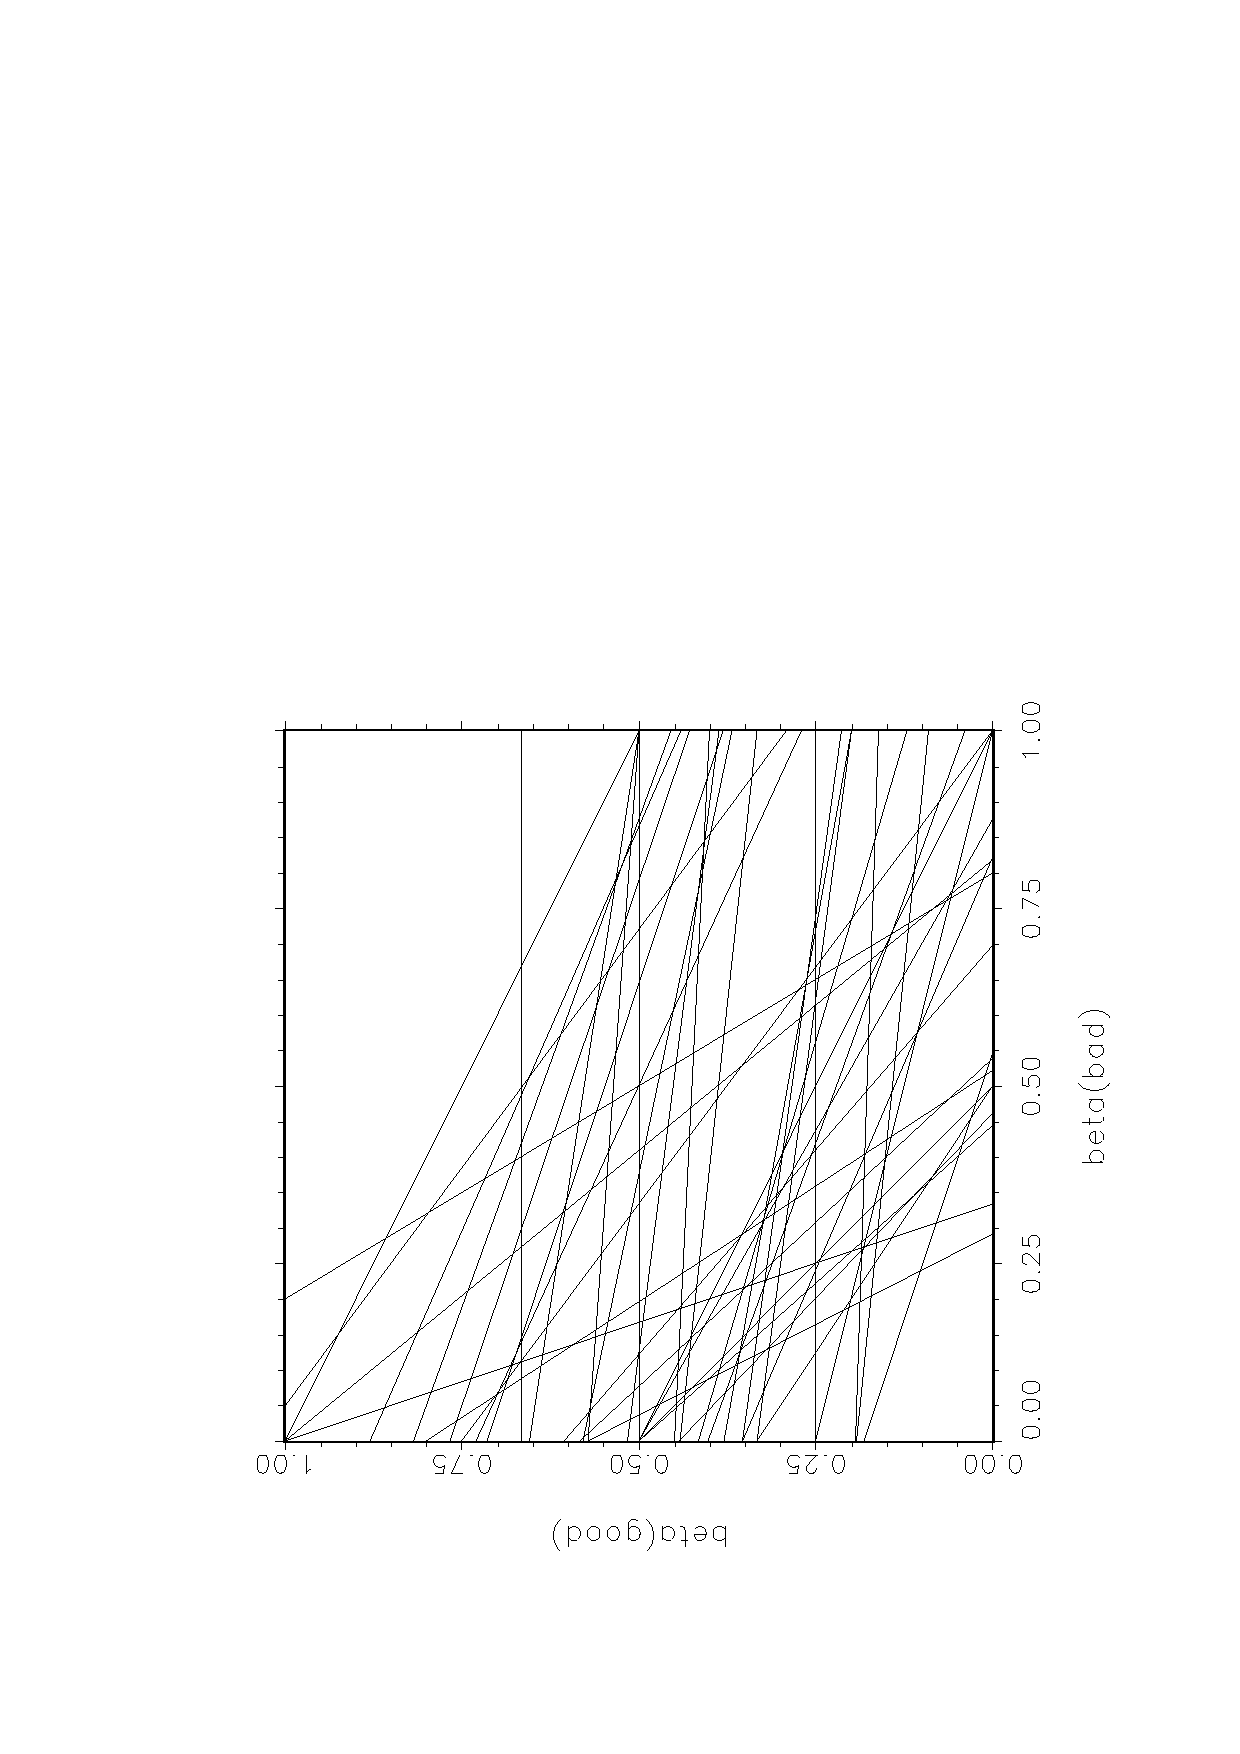
\includegraphics[width=2.25in,height=3in,angle=-90]{tomog}
%     \end{center}
%   \end{minipage}
%   \caption{\small \label{fg:tomog} Tomography Plot for Florida Counties.}
% \end{figure}

\begin{minipage}[b]{0.5\linewidth} % A minipage that covers half the page
  \centering \color{Red}
  \begin{equation*}
    \text{Citrus County: $T=.13$, $X=.25$} 
  \end{equation*}
  \begin{align*}
    \bg_i &= \frac{T_i}{1-X_i}-\frac{X_i}{1-X_i}\bb_i\\
    &= \frac{.13}{1-.25}-\frac{.25}{1-.25}\bb_i\\
    &= .173 - .333\bb_i
  \end{align*}
\end{minipage}
\hspace{0.5cm} % To get a little bit of space between the figures
\begin{minipage}[b]{0.5\linewidth}
  \centering
  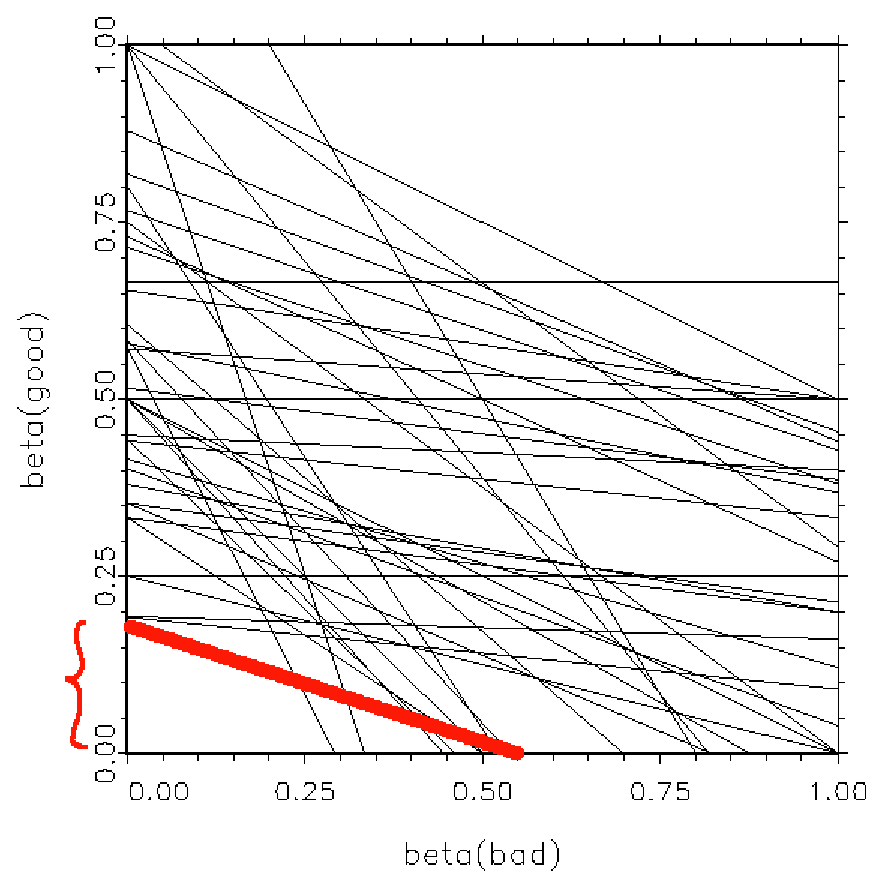
\epsfig{file=tomogc.eps, width=2in}
\end{minipage}

\end{slide}

%%%%%%%%%%%%%%%%%%%%%%%%%%%%%%%%%%%%%%%%%%%%%%%%%%%%%%%%%%%%%%%%%%%

\begin{slide}
\heading{Analysis of Bounds}
\bigskip

\smallskip
\begin{table}
\begin{center}
\begin{tabular}{l |ccc|ccc| c}
  & \multicolumn{3}{c|}{\bf Gore's votes} &
  \multicolumn{3}{c|}{\bf Bush's votes} & \bf Total   \\
   & official & \multicolumn{2}{c|}{\textcolor{Red}{invalid ballots}} & official &
  \multicolumn{2}{c|}{\textcolor{Red}{invalid ballots}} & invalid\\
County  & count & \textcolor{Red}{min} & \textcolor{Red}{max} & count & \textcolor{Red}{min} & \textcolor{Red}{max} & ballots\\
\hline 
Baker      &  0 & \textcolor{Red}{0} & \textcolor{Red}{0} &   1 &  \textcolor{Red}{1} &   \textcolor{Red}{1} &   1 \\
Escambia   & 47 & \textcolor{Red}{0} & \textcolor{Red}{47} & 154 & \textcolor{Red}{48} & \textcolor{Red}{102} & 102 \\
Santa Rosa & 16 & \textcolor{Red}{0} & \textcolor{Red}{16} &  65 & \textcolor{Red}{37} &  \textcolor{Red}{55} &  55 \\
$\vdots$ & $\vdots$ &
$\textcolor{Red}{\vdots}$ & $\textcolor{Red}{\vdots}$ &
$\vdots$ & $\textcolor{Red}{\vdots}$ &
$\textcolor{Red}{\vdots}$ & $\vdots$ \\
\hline
\bf all counties  & \bf 836 & \bf \textcolor{Red}{5} & \bf \textcolor{Red}{527} & \bf 1575 & \bf \textcolor{Red}{128} & \bf \textcolor{Red}{668} & \bf 680\\ 
\end{tabular} 
\end{center}
\end{table} 

\begin{center}
  {\bf Bush's margin without bad ballots} $\in \textcolor{Red}{[-126, 936]}$
\end{center}

\end{slide}

%%%%%%%%%%%%%%%%%%%%%%%%%%%%%%%%%%%%%%%%%%%%%%%%%%%%%%%%%%%%%%%%%%%

\begin{slide}
\heading{Statistical Modeling}
\bigskip

{\bf Key Assumptions of EI}
\begin{itemize}
\item Systematic differences in $\bb_i$ and $\bg_i$ are accounted
  for by covariates.
\item Conditional on covariates, there is no spatial correlation.
\item Conditional on covariates, $\bb_i$ and $\bg_i$ are independent
  of $X_i$. 
\end{itemize}

\bigskip
{\bf Difficulties of Ecological Inference}
\begin{itemize}
\item Sensitivity: Estimation results can be sensitive to model
  specification when bounds are wide.
\item Weak identifiability: We cannot include many covariates in one model.
\end{itemize}

\bigskip
{\bf Particular Challenges of this Study}
\begin{itemize}
\item No strong theoretical guidance for model choice.
\item Need to build models not vulnerable to criticism from partisans.
\end{itemize}

\end{slide}

%%%%%%%%%%%%%%%%%%%%%%%%%%%%%%%%%%%%%%%%%%%%%%%%%%%%%%%%%%%%%%%%%%%

\begin{slide}
\heading{Bayesian Model Averaging}

{\bf Data and Model:} 31 models using covariates including $X_i$,
race, sex, party registration for the absentee voters, county level
election results, and demographic variables.

{\bf Bayesian Inference:} 
$\textcolor{Purple}{\P(\Delta|T,M)} \propto \P(\Delta|M)\P(T|\Delta,M).$

{\bf Model Averaging:} 
\begin{equation*}
\Pr(\Delta|T) 
 = \sum_{k=1}^{31} \textcolor{Purple}{\P(\Delta|M_k,T)} \textcolor{Red}{\Pr(M_k|T)}
\end{equation*}

\textcolor{Red}{{\bf Posterior Model Probability:}}
\begin{itemize} 
\item The probability of the model, $k$, being true given the data.
\item Different from measures of fit like $R^2$.
\item Computed via the Bayes Theorem
  \begin{equation*}
    \textcolor{Red}{\Pr(M_k|T)} =  \frac{\P(T|M_k)\Pr(M_k)}{\sum_{j=1}^{31} \Pr(T|M_j) \Pr(M_j)}.  
  \end{equation*}
\end{itemize}


\end{slide}

%%%%%%%%%%%%%%%%%%%%%%%%%%%%%%%%%%%%%%%%%%%%%%%%%%%%%%%%%%%%%%%%%%%

\begin{slide}
\centerline{\textbf{\small Probability that Gore Would Have Won Without Flawed Ballots}}

\begin{figure}
\begin{center}
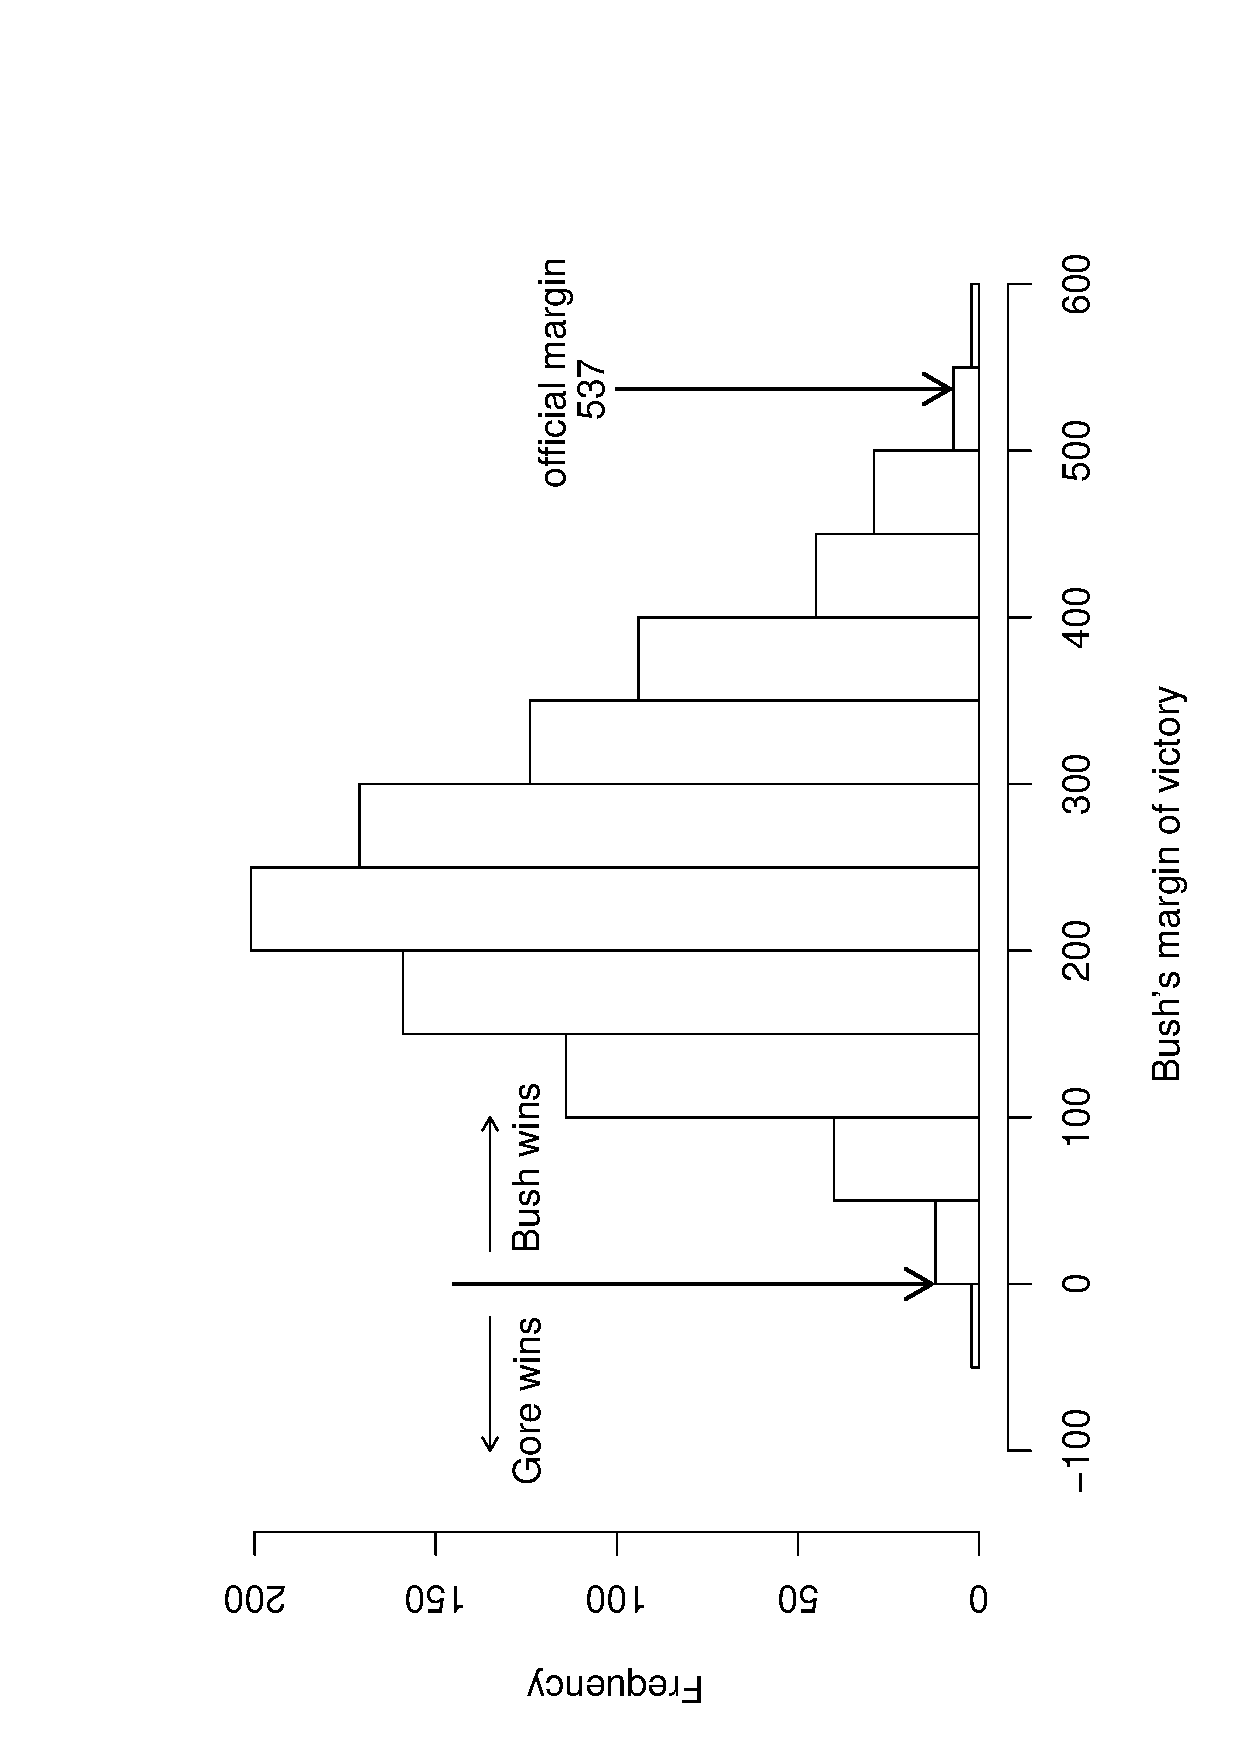
\includegraphics[width=2.5in,height=4in,angle=-90]{margin}
\caption{\small Posterior distribution of Bush's margin of victory without the
  680 invalid overseas absentee ballots} \label{fg:margin}
\end{center} 
\end{figure}
\end{slide}

%%%%%%%%%%%%%%%%%%%%%%%%%%%%%%%%%%%%%%%%%%%%%%%%%%%%%%%%%%%%%%%%%%%

\begin{slide}
\heading{Other Counterfactuals}

\begin{table}
\small
\begin{center}
\begin{tabular}{l..}
 & \multicolumn{1}{c}{Bush's margin} & \multicolumn{1}{c}{Prob(Gore Wins)}\\
\hline
Invalid overseas ballots alone & 251  & 0.002 \\
\emph{Actual recounts}\\
\hspace{1em} Miami Dade partial recount     &  94  & 0.19 \\
\hspace{1em} Palm Beach recount             &  59  & 0.29 \\
\hspace{1em} Miami Dade and Palm Beach    & -98  & 0.82 \\
\emph{Media recounts}\\
\hspace{1em} No U.S.\ Supreme Court decision  & 242  & 0.01\\
\hspace{1em} Gore's request granted         & -26  & 0.73\\
\hspace{1em} only fully punched ballots     & -366 & >0.99 \\
\hspace{1em} hanging chads and dimples      & -358 & >0.99 \\
\hspace{1em} each county's standard         & -422 & >0.99 \\
\end{tabular}
\end{center}
\caption{\small Estimated margin and probability of victory with selected
counterfactuals} \label{tb:senario}
\end{table}
\normalsize
\end{slide}

%%%%%%%%%%%%%%%%%%%%%%%%%%%%%%%%%%%%%%%%%%%%%%%%%%%%%%%%%%%%%%%%%%%

\begin{slide}
\heading{Indirect Evidence of Local Election Officials} 
\heading{Responding to Republican Pressure}
\bigskip

\begin{itemize}
\item The \emph{New York Times} concluded ``Their [Republicans'] goal was
simple: to count the maximum number of overseas ballots in counties
won by Mr.  Bush, particularly those with a high concentration of
military voters, while seeking to disqualify overseas ballots in
counties won by Vice President Al Gore.''

\bigskip
\item The \emph{Times} claimed that as a direct result of this pressure,
``canvassing boards in about a dozen Republican-leaning counties had
reconvened for a second round of counting.  In each place,
longstanding election rules were bent and even ignored.  Boards
counted ballots postmarked as many as seven days after the election,
including some from within the United States.  They counted two
ballots sent by fax.  Officials in Santa Rosa County even counted five
ballots that arrived after the Nov.\ 17 deadline.  Again and again,
election officials crossed out the words `REJECTED AS ILLEGAL' that
had been stamped on ballot envelopes.''
\end{itemize}
  
\end{slide}

%%%%%%%%%%%%%%%%%%%%%%%%%%%%%%%%%%%%%%%%%%%%%%%%%%%%%%%%%%%%%%%%%%%

\begin{slide}
\begin{table}
\footnotesize
\begin{tabular}{l....|.}
& \multicolumn{1}{c}{military} 
& \multicolumn{1}{c}{Republican} 
& \multicolumn{1}{c}{\textcolor{Purple}{Bad ballot}}
& \multicolumn{1}{c}{\textcolor{Purple}{Bad Ballots}}
\\ 
& \multicolumn{1}{c}{ballots} 
& \multicolumn{1}{c}{vote} 
& \multicolumn{1}{c}{\textcolor{Purple}{acceptance}}
& \multicolumn{1}{c}{\textcolor{Purple}{counted for Bush}}
& \multicolumn{1}{c}{all ballots}\\    \hline
    \multicolumn{4}{l}{\bf Republican pressure to count} \\
    \hspace{1em}Collier  & 46.7\% & 65.6\% & \textcolor{Purple}{53}.\textcolor{Purple}{7\%} & \textcolor{Purple}{64}.\textcolor{Purple}{5\%} & 60 \\    
    \hspace{1em}Duval    & 83.8 & 57.5 & \textcolor{Purple}{62}.\textcolor{Purple}{3} & \textcolor{Purple}{67}.\textcolor{Purple}{8} & 637 \\
    \hspace{1em}Escambia & 88.6 & 62.6 & \textcolor{Purple}{64}.\textcolor{Purple}{2} & \textcolor{Purple}{80}.\textcolor{Purple}{3} & 272 \\         
    \hspace{1em}Okaloosa & 88.9 & 73.7 & \textcolor{Purple}{42}.\textcolor{Purple}{0} & \textcolor{Purple}{69}.\textcolor{Purple}{4} & 189 \\          
    \hspace{1em}Pasco    & 62.3 & 48.0 & \textcolor{Purple}{60}.\textcolor{Purple}{5} & \textcolor{Purple}{76}.\textcolor{Purple}{4} & 53 \\                
    \hspace{1em}Santa Rosa & 90.3 & 72.1 & \textcolor{Purple}{84}.\textcolor{Purple}{6} & \textcolor{Purple}{84}.\textcolor{Purple}{4} & 93 \\
    \hspace{1em}\emph{Average} & \emph{83}.\emph{4} & \emph{60}.\emph{0} & \textcolor{Purple}{\emph{61}}.\textcolor{Purple}{\emph{5}} & \textcolor{Purple}{\emph{74}}.\textcolor{Purple}{\emph{3}} & 1304 \\
\multicolumn{5}{l}{\bf Counties not mentioned by the \emph{Times}}
& \\ 
\hspace{1em}\emph{Average} & \emph{67}.\emph{6} & \emph{51}.\emph{8} & \textcolor{Purple}{\emph{30}}.\textcolor{Purple}{\emph{0}} & \textcolor{Purple}{\emph{71}}.\textcolor{Purple}{\emph{5}} & 1751\\
\multicolumn{4}{l}{\bf Republican pressure not to count}\\ 
    \hspace{1em}Alachua    & 46.8 & 39.8 & \textcolor{Purple}{12}.\textcolor{Purple}{5} & \textcolor{Purple}{54}.\textcolor{Purple}{5} & 77 \\ 
    \hspace{1em}Broward    & 46.9 & 30.9 & \textcolor{Purple}{21}.\textcolor{Purple}{8} & \textcolor{Purple}{54}.\textcolor{Purple}{3} & 213 \\  
    \hspace{1em}Miami Dade & 44.4 & 46.3 & \textcolor{Purple}{11}.\textcolor{Purple}{7} & \textcolor{Purple}{57}.\textcolor{Purple}{1} & 306 \\
    \hspace{1em}Palm Beach & 45.3 & 35.3 & \textcolor{Purple}{40}.\textcolor{Purple}{7} & \textcolor{Purple}{56}.\textcolor{Purple}{2} & 53 \\ 
    \hspace{1em}\emph{Average} & \emph{45}.\emph{6} & \emph{38}.\emph{1} & \textcolor{Purple}{\emph{17}}.\textcolor{Purple}{\emph{2}} & \textcolor{Purple}{\emph{55}}.\textcolor{Purple}{\emph{4}} &  649 \\
    \hline                                                       
  \end{tabular}                                                
  \caption{\footnotesize Counties classified by whether the \emph{Times} reported evidence of Republican pressure.} 
\end{table}

\end{slide}

%%%%%%%%%%%%%%%%%%%%%%%%%%%%%%%%%%%%%%%%%%%%%%%%%%%%%%%%%%%%%%%%%%%

\begin{slide}
\heading{Qualitative Evidence Backs Up Statistical Analysis}
\bigskip

\begin{itemize}
\item An election official on the Duval County canvassing board ``held
  the line on counting ballots with missing postmarks.''

\bigskip
  
\item ```It looks to me like we've got a lot of pressure here,' Judge
  Robert P.  Cole, chairman of the Pasco board, said as he faced a
  throng of cheering Republicans and more than a dozen Bush
  representatives [and no officials from the Gore campaign].''
\end{itemize}

\end{slide}

%%%%%%%%%%%%%%%%%%%%%%%%%%%%%%%%%%%%%%%%%%%%%%%%%%%%%%%%%%%%%%%%%%%

\begin{slide}
\heading{Results of Bayesian Model Averaging}
\small
\begin{table}
\begin{center}
\begin{tabular}{l c r@{, }l d{3} d{-3}}
  & \multicolumn{3}{c}{Bush's margin}& \multicolumn{1}{c}{first} 
  & \multicolumn{1}{c}{Posterior model} \\
  & \multicolumn{3}{c}{(95 \% C.I.)} & \multicolumn{1}{c}{difference} 
  & \multicolumn{1}{c}{probability} \\
\hline
\multicolumn{1}{l}{Bayesian Model Averaging} & 251 & (69 & 468) & \\
\multicolumn{1}{l}{\emph{Individual models}}  \\ 
\hspace{0.5em} Registered Repub.\ absentee voters
 & 269 & (97 & 475) & $-52$ &  0.565 \\
\hspace{0.5em} Dem.\ vote share
 & 232 & (69 & 448) & 3 &  0.239 \\
\hspace{0.5em} Black absentee voters
 & 231 & (69 & 440) & $-2$ &  0.102 \\
\hspace{0.5em} White absentee voters
 & 123 & ($-$18& 315) & $-23$ &  0.033 \\
\hspace{0.5em} Registered black Repubs
 & 229 & (62 & 441) & $-6$ &  0.021 \\
\hspace{0.5em} Accepted absentee ballots
 & 218 & (62 & 409) & 4 &  0.004 \\
\end{tabular}
\caption{Estimates of Bush's margin of victory after dropping the
  invalid overseas absentee ballots.}
\label{tb:bma}
\end{center}
\end{table}

\end{slide}

%%%%%%%%%%%%%%%%%%%%%%%%%%%%%%%%%%%%%%%%%%%%%%%%%%%%%%%%%%%%%%%%%%%

\begin{slide}
\heading{Model Fit}

\begin{figure}
\hspace{0.5in}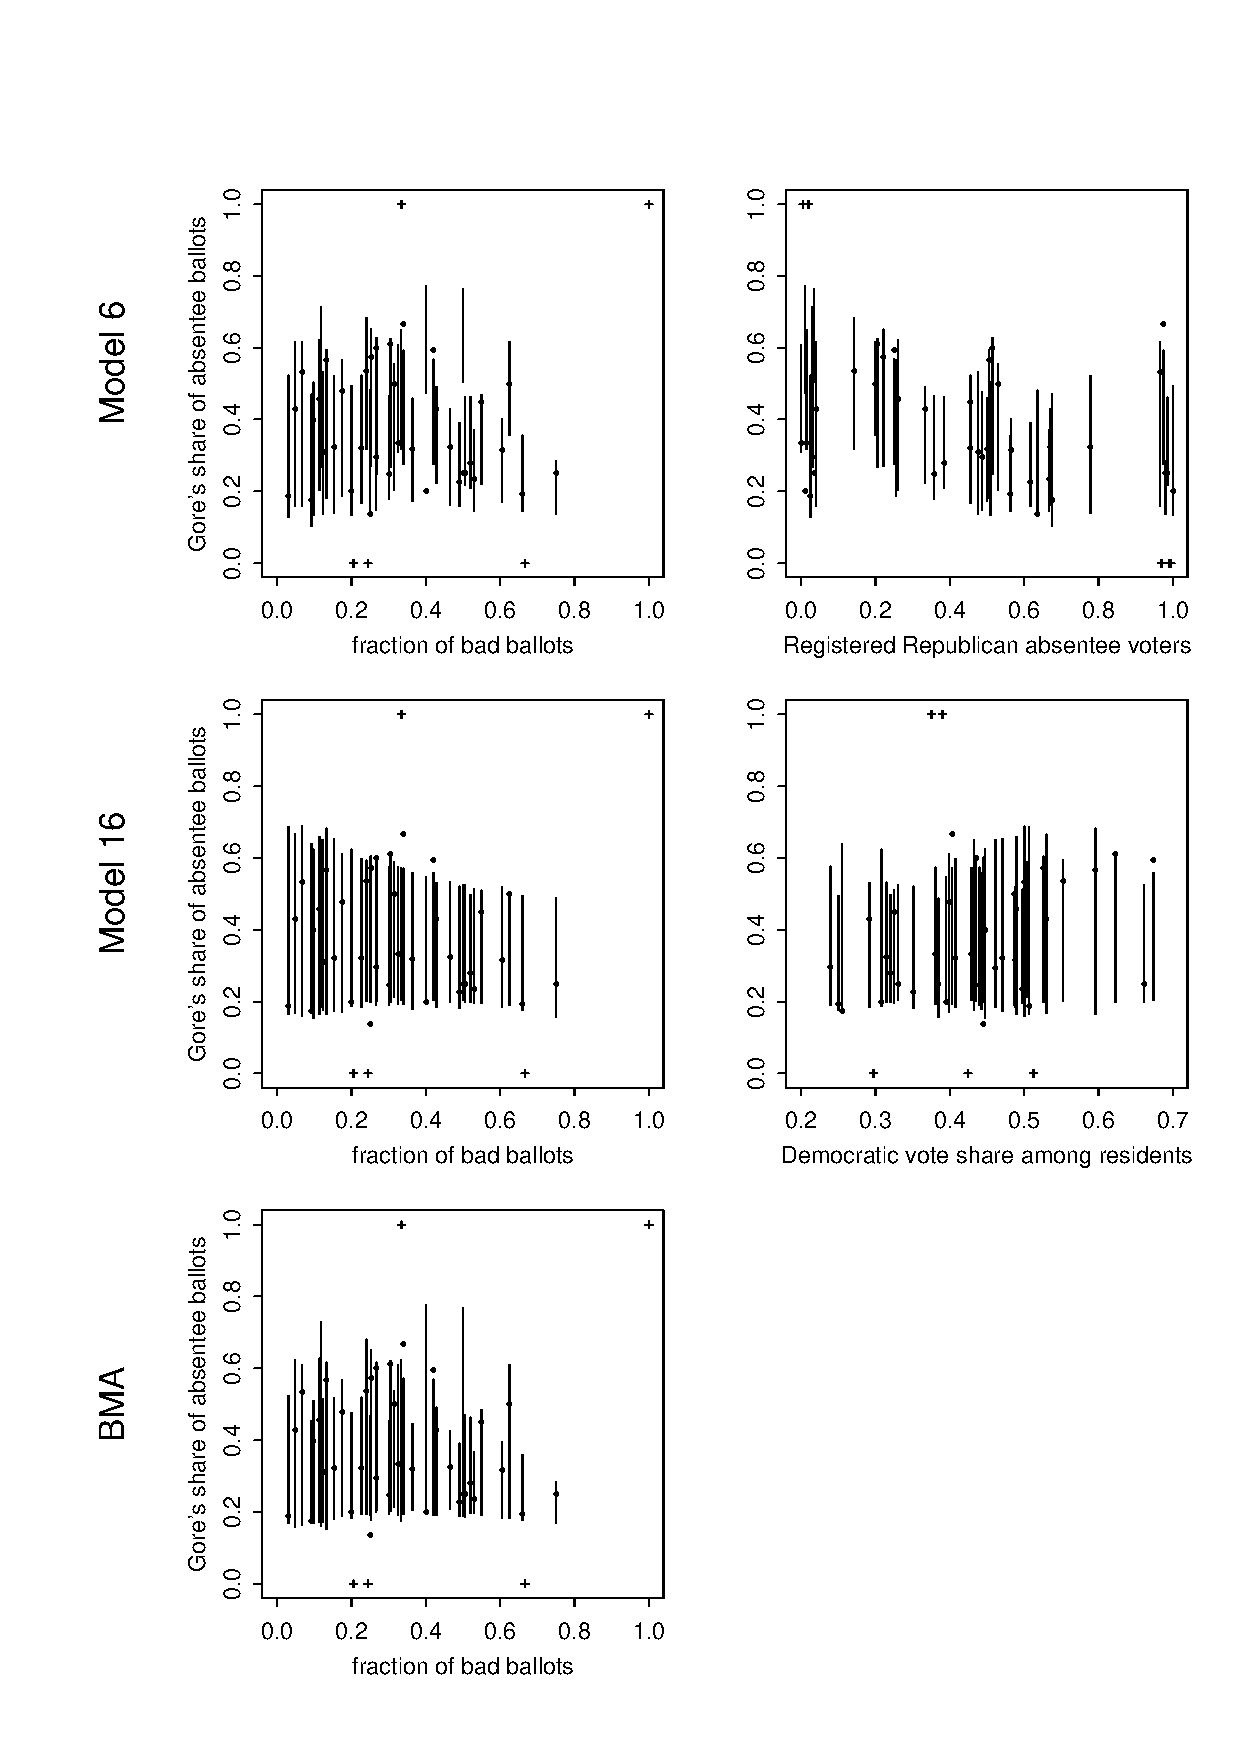
\includegraphics[width=4in,height=3in]{fit}
\caption{\small Posterior predicted distribution of $T_i$, (80\%
  confidence intervals).}
\end{figure}
\end{slide}

%%%%%%%%%%%%%%%%%%%%%%%%%%%%%%%%%%%%%%%%%%%%%%%%%%%%%%%%%%%%%%%%%%%

\begin{slide}
\heading{Sensitivity Analysis}
\begin{figure}
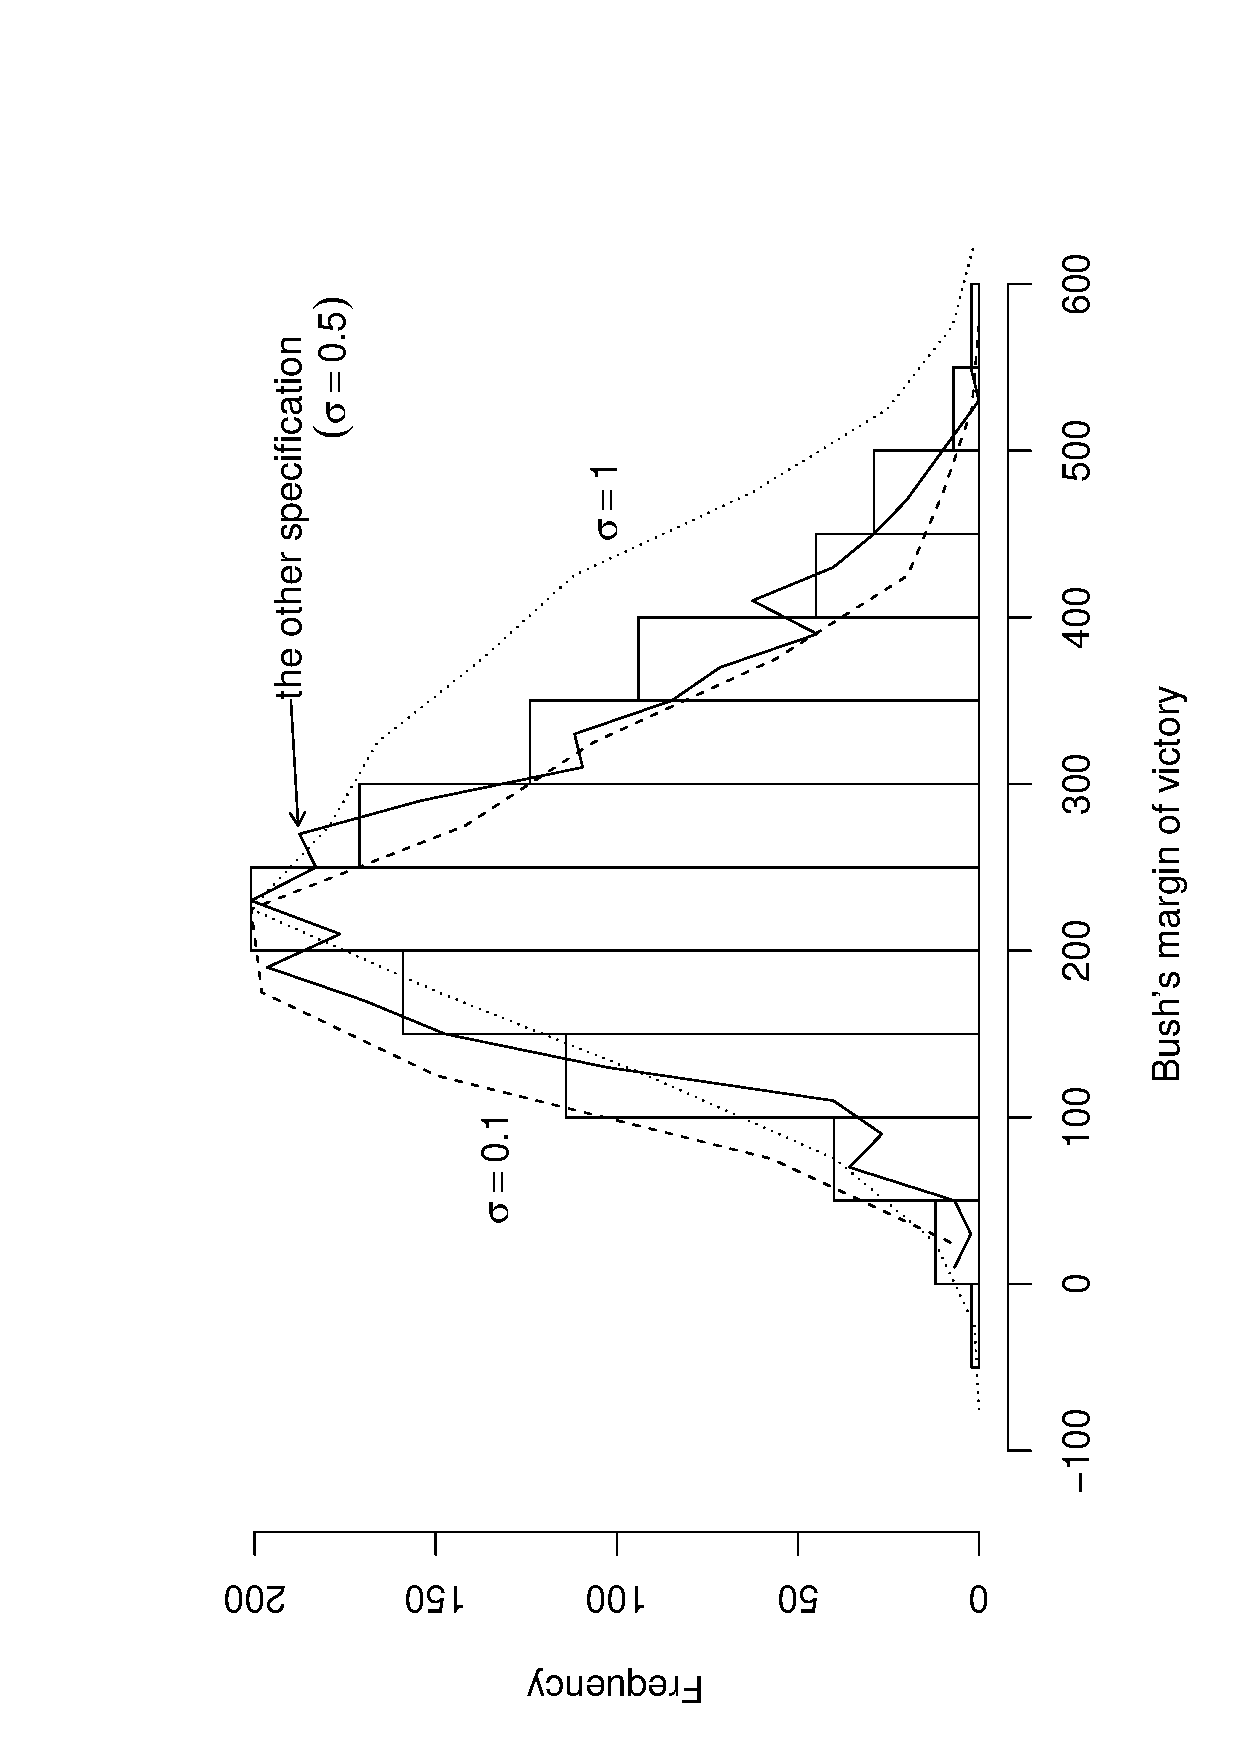
\includegraphics[width=3in,height=4.5in,angle=-90]{sensitivity}
\caption{\small Sensitivity analysis of Bayesian model averaging.}
\end{figure}
\end{slide}

%%%%%%%%%%%%%%%%%%%%%%%%%%%%%%%%%%%%%%%%%%%%%%%%%%%%%%%%%%%%%%%%%%%

\begin{slide}
\heading{Concluding Remarks}
\bigskip

\begin{enumerate}
\item Voter intentions aside, who won according to the law?  
  \begin{enumerate}
  \item We will never know for certain.
  \item Bush probably won, fixing only the bad ballot problem
  \item Almost any other scenerio would have probably led to a Gore
    victory
  \end{enumerate}
  
\item Quantitative evidence confirms qualitative stories of Republican
  pressure (which is fine) and local election officials responding
  (which is not).
  
\item Our counterfactual questions are very close to the data and
  easier to validate.
\item First political science application of formal Bayesian model averaging.
\item First use of Bayesian model averaging in the growing ecological
  inference literature.
\item An approach towards the uncertainty of model choice.
\item Model averaging cannot substitute for the investigator's
  judgment.
\end{enumerate}

\end{slide}

\end{document}


